%appendix A
\chapter{Arborescences}\label{arbo}

\begin{figure}[h]
\begin{center}
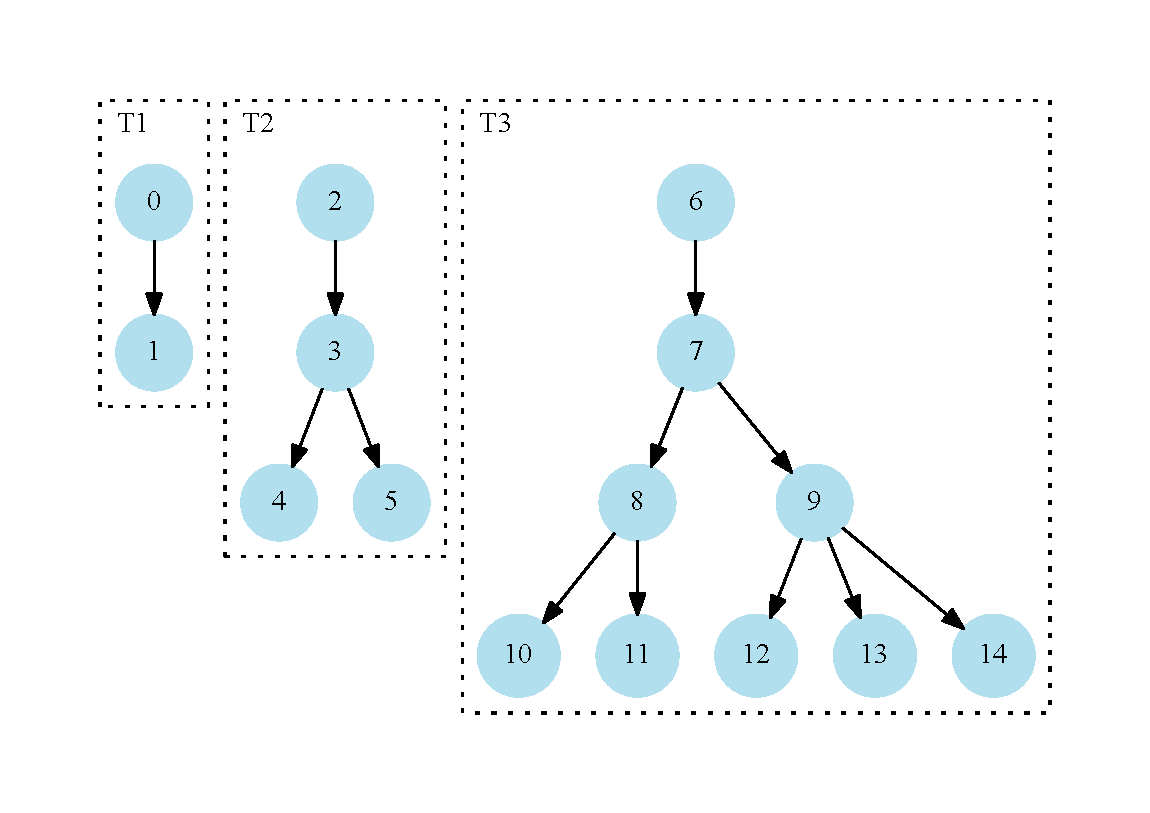
\includegraphics[scale=0.6]{./images/t1_2_3.pdf}
\end{center}
\caption{arborescences $T_1$, $T_2$, $T_3$}
\end{figure}
\clearpage

\begin{figure}[h]
\begin{center}
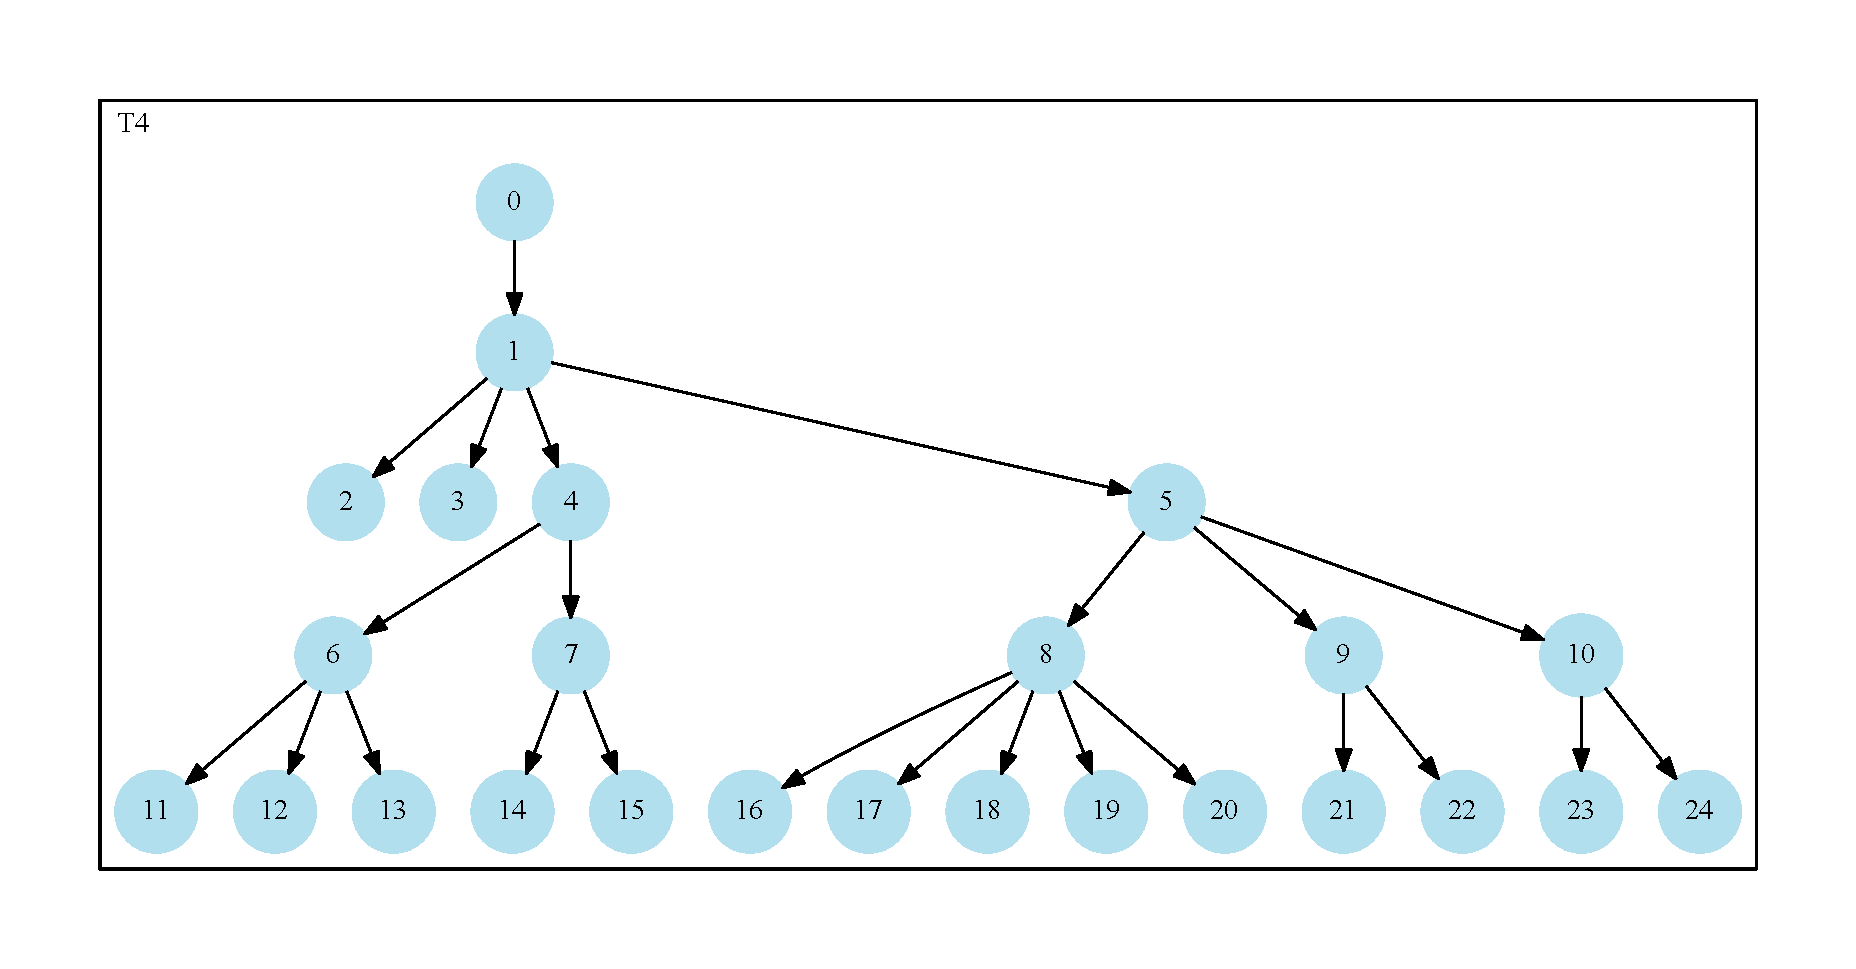
\includegraphics[scale=0.4]{./images/t4.pdf}
\end{center}
\caption{arborescence $T_4$}
\end{figure}
\clearpage

\chapter{Programmation}

\begin{rem}[astuce -- trafic automobile]
En C/C++, on peut repr\'esenter une s\'equence de $n$ bits par un entier non sign\'e de type \verb+uint32_t+ dont on ne consid\`ere que les $n$ premiers bits \`a droite dans l'\'ecriture en base 2. On peut alors coder $f$ facilement en utilisant des op\'erations de \og masques \fg{} (symboles \verb+&+, \verb+|+, \verb+!+, \verb+^+) et de d\'ecalage de bits (symboles \verb+<<+ et \verb+>>+) qui correspondent respectivement \`a des op\'erations logiques bit-\`a-bit et \`a des divisions/multiplications par des puissances de 2. Nous renvoyons au code de la fonction $f$ qui tient en une seule ligne.
\end{rem}